
\documentclass[12pt]{report}
\usepackage{titlesec}
\usepackage[utf8]{inputenc}
\usepackage[T1]{fontenc}
\usepackage[english]{babel}

\usepackage{graphicx}
\graphicspath{{images/}}
\usepackage{float}


\usepackage{natbib}
\bibliographystyle{agsm}


\usepackage[hidelinks]{hyperref}

\usepackage{amsmath}
\usepackage{amsfonts}
\usepackage{amssymb}

\usepackage[a4paper, width=150mm, top=25mm, bottom=25mm]{geometry}
\usepackage{setspace}
\usepackage{fancyhdr}
\pagestyle{fancy}

\titleformat{\chapter}[display]
{\normalfont\bfseries}{}{0pt}{\Huge}


\begin{document}
  
  \begin{titlepage}
    \begin{center}
      \vspace{1em}
	  \large{Master Thesis}\\
	  \huge Gaining Customer Insights using Machine Learning on Graphs \\ 
	  \large \vspace{1em}
	  University of Basel\\
	  \vspace{4em}
	  \large
	  Author: \\
	  Michael von Siebenthal\\
	  \vspace{2em}
	  Supervisor: \\
	  Prof. Dr. Dietmar Maringer\\
	  \vspace{2em}
	  \today
	  \vspace{3em}
    \end{center}
  \end{titlepage}



  %%% frontmatter
  \chapter*{Abstract}
  Abstract goes here

  \chapter*{Declaration}
    "I hereby declare - that I have written this master thesis without any help 
  from others and without the use of documents and aids other than those stated 
  in the references, - that I have mentioned all the sources used and that I 
  have cited them correctly according to the established academic citation rules, 
  - that the topic or part of it are not already the object of any work or 
  examination of another course unless explicitly stated,- that I am aware of 
  the consequences of plagiarism at the Business and Economics Faculty of University of Basel."\\\\\\\\\\
  Michael von Siebenthal, Martikel-Nr.: 2015-256-837, Date: \today


  \tableofcontents
  \listoffigures
  \listoftables

  %%% Main Body
  \onehalfspacing
  
  % Introduction
  \chapter{Introduction}
  	
	This thesis investigates models for gaining customer insights using graph
	machine learning. Graph machine learning is a current frontier in machine 
	learning and has many successful applications in many areas such as recently 
	shown by the success of AlphaFold \citep{senior2020improved}. AlphaFold made 
	a breakthrough for predicting protein structures where they made use of the 
	observation that a folded protein can be considered as a spatial graph 
	\citep{AlphaFoldTeam2020}. More generally, there are a vast range of 
	applications for graph machine learning in the fields of natural science, 
	social science and many more as shown by the excellent overview given by 
	\cite{zhou2020graph}. Graphs are especially useful as they allow for the 
	consideration of relationships between observations. Graph machine learning 
	has for that reason become a promising field as it allows for the use of
	richer data. This thesis will focus on graph machine learning for the
	purpose of customer classification. In particular, it is investigated to
	what extent semi-synthetic graphs can be used for graph machine learning.
	To provide a better overview as to how this topic relates to business \& 
	economics related fields such as gaining customer insights, some motivating
	examples are provided in the following section. 
	
	\section{Relevance to Economics}

	\noindent From a business \& economics perspective, graphs are particularly
	interesting if one wants to model the interactions between institutions. An 
	example for this is shown in an article published by 
	\cite{schweitzer2009economic} which created the graph shown in figure
	\ref{fig:bank_network}. This graph depicts the interdependencies of 
	international banks. Such graphs can be useful tools for analyzing such 
	interdependencies and to provide important information for making the banking 
	system more robust and resilient. 

	\begin{figure}[h]
		\centering
		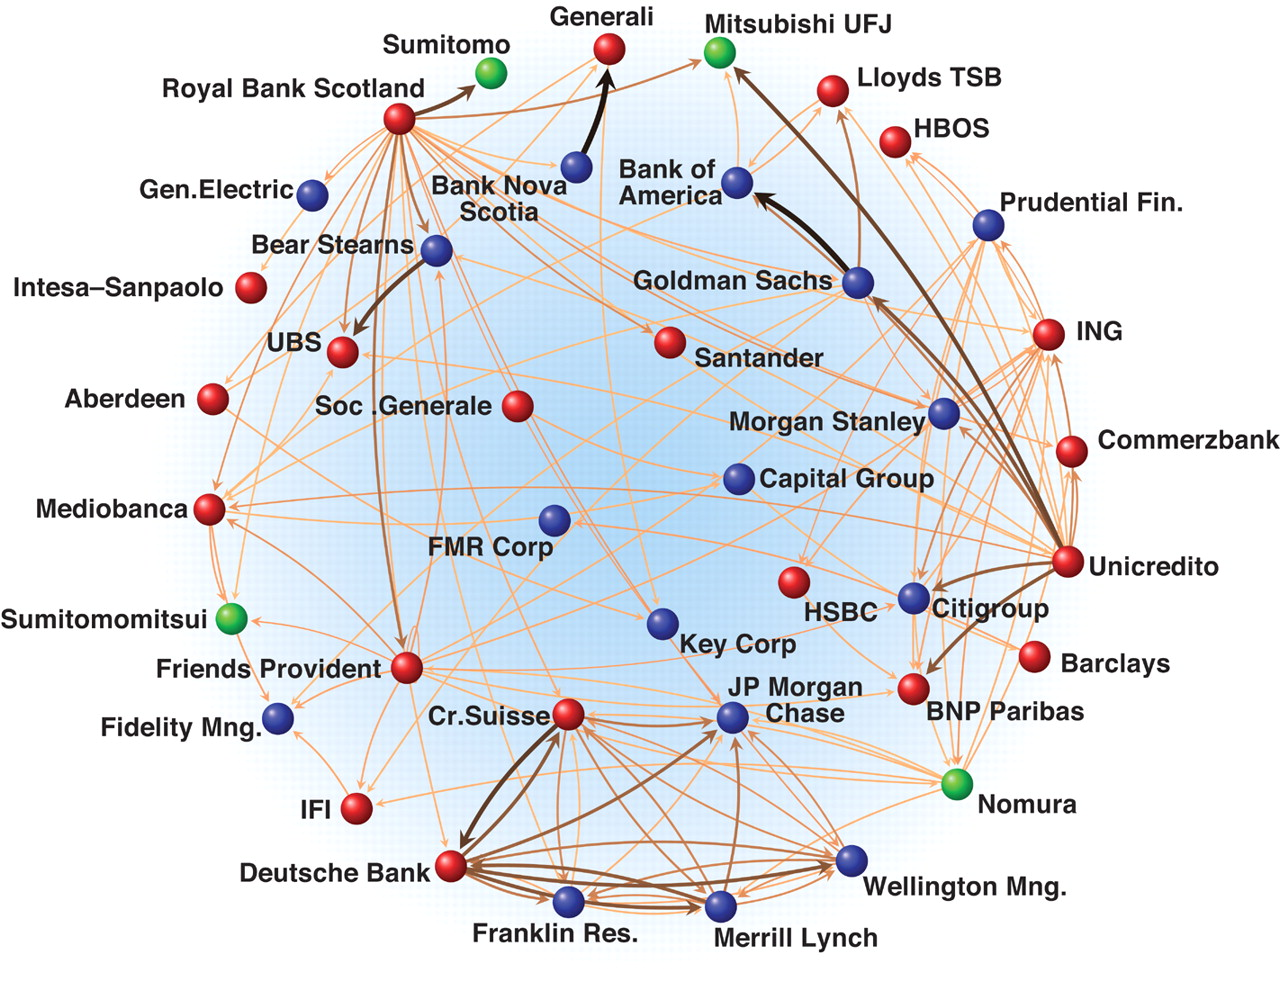
\includegraphics[width=0.5\textwidth]{bank_network.jpg}
		\caption{Bank Network}
		\cite[p. 424]{schweitzer2009economic}
		\label{fig:bank_network}
	\end{figure} 

	\noindent Another interesting application of graphs is to model social 
	interactions. While there are many different areas of interest which make
	use of social connections, the focus of this thesis is placed on gaining 
	customer insights. Indeed, this is one of the main areas where social network 
	companies such as Facebook or search providers like Google make their
	revenue. Those companies mainly generate their revenue by providing customer 
	insights or selling targeted advertising \citep{Facebook2021,Alphabet2021}. 
	Both Facebook and Google have the advantage, that their businesses naturally 
	capture relational or more generally network data. Most researchers and 
	companies however do not have access to such data. Companies for instance 
	may have access to large amounts of customer data. This data however 
	typically does not contain relational information (e.g. which client is 
	connected with which other clients). The same is true for researchers, where 
	social scientists often collect data via anonymous surveys. This makes the 
	collection of network data basically impossible. For that reason, most 
	companies and researchers are limited to working with data such as 
	cross-sectional data that contain no network information. It is important 
	to mention, that there is a lot of network data available online. This 
	network data however typically only contains the network connections. The 
	important feature data such as demographic data, topic specific variables 
	and labels are however typically not available. Without feature data, graphs 
	provide rather limited information for gaining customer insights. 
	This is a data access and data collection problem and is a frustrating 
	reality which also affects this master's thesis. It however motivates the 
	research topic which is presented in section \ref{section:research_topics}. 
	First, a general overview of machine learning is given in the following 
	section.
	
	\section{Overview Machine Learning}

	This section provides a high-level overview of machine learning and
	specifies the type of machine learning task used for this thesis. To
	start, it is important to correctly categorize machine learning. There are
	many related big topics such as data science, big data or artificial
	intelligence and it is often not clear what exactly is meant. An overview
	of how these different terms can be categorized is shown in figure 
	\ref{fig:ml_overview}.

	\begin{figure}[h]
		\centering
		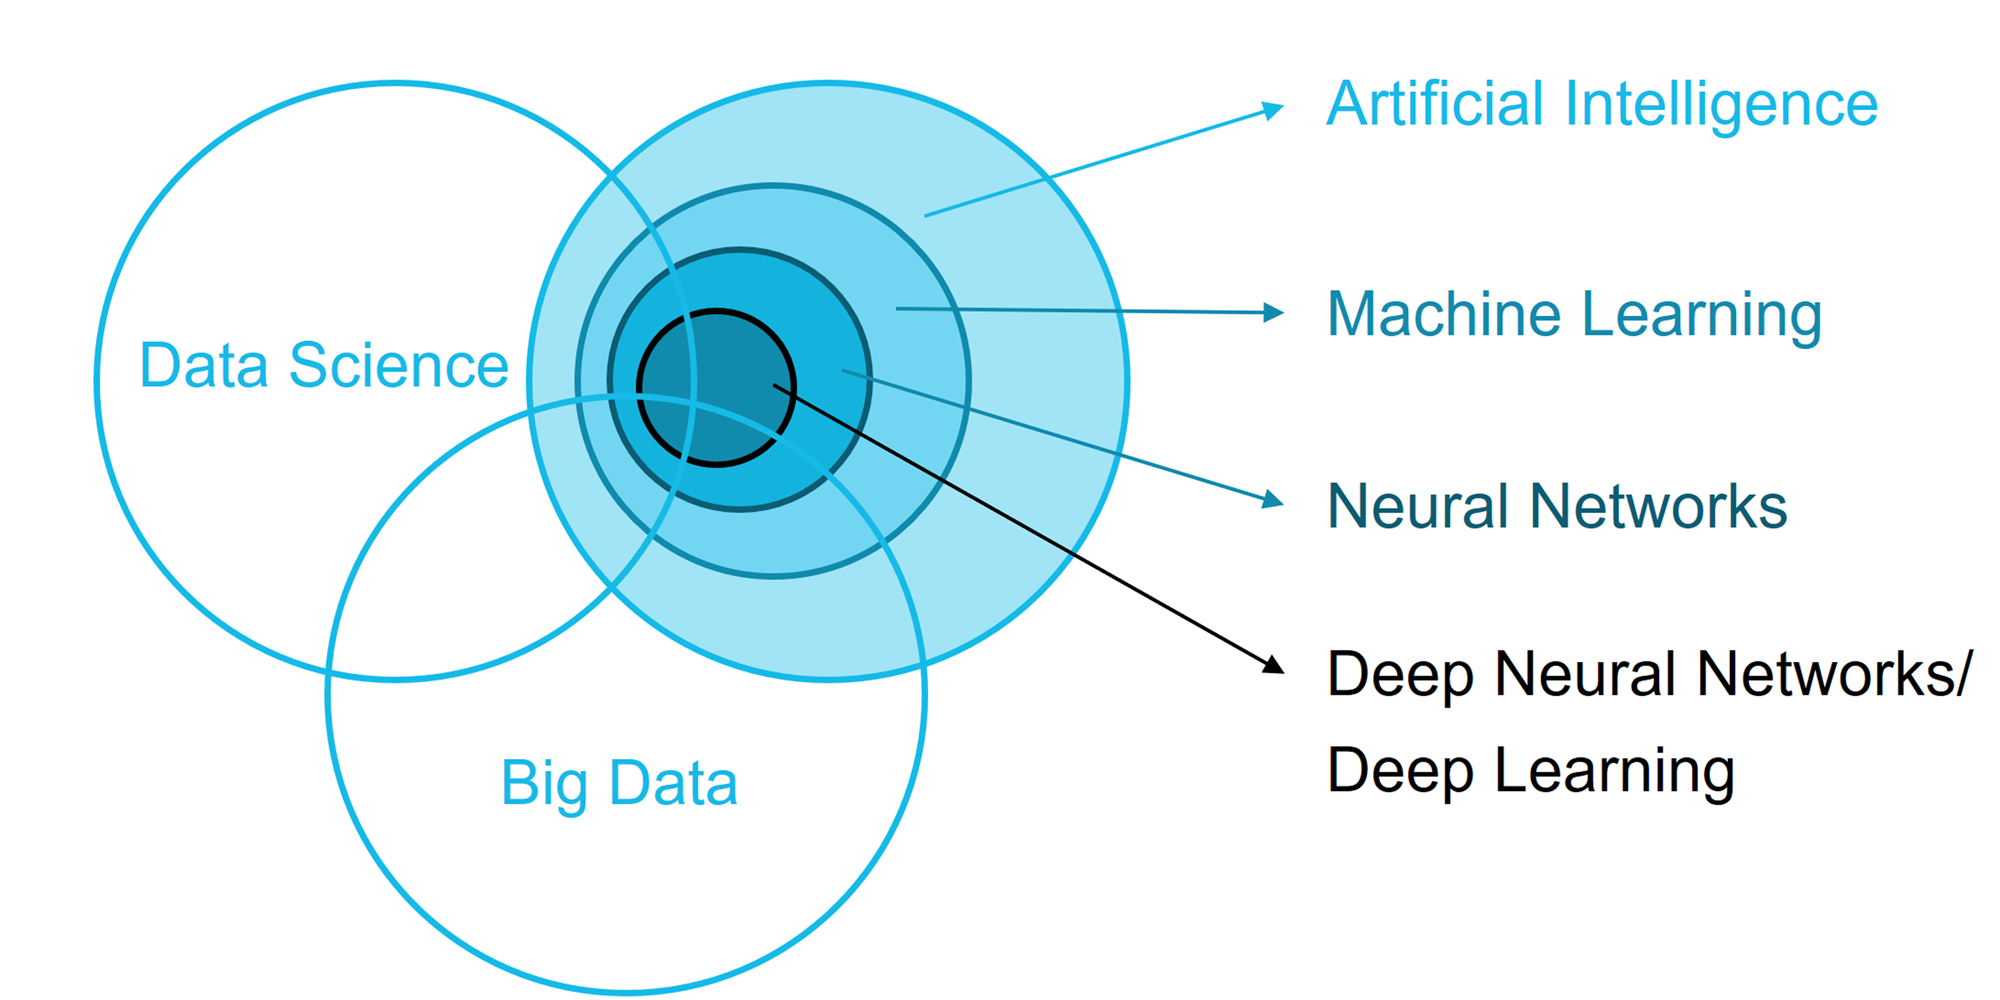
\includegraphics[width=0.7\textwidth]{overview_datascience.png}
		\caption{Overview Machine Learning}
		\citep{Frauenhofer2021}
		\label{fig:ml_overview}
	\end{figure} 

	\noindent Figure \ref{fig:ml_overview} shows well, how these different
	terms are related with each other. Machine learning in particular is
	mostly ascribed to the domain of artificial intelligence. It however also 
	has a shared domain with data science and big data. It is thus at the
	intersection of these three interrelated fields. Machine learning models 
	such as neural networks and deep neural networks are specific models within
	machine learning and are often referred to separately due to their
	popularity. In this thesis, differentiating between machine learning and
	neural networks is not necessary, as the considered machine learning models
	are used for the same task. Machine learning can be applied for various
	tasks and is again best presented visually as shown in figure 
	\ref{fig:ml_tasks}.

	\begin{figure}[h]
		\centering
		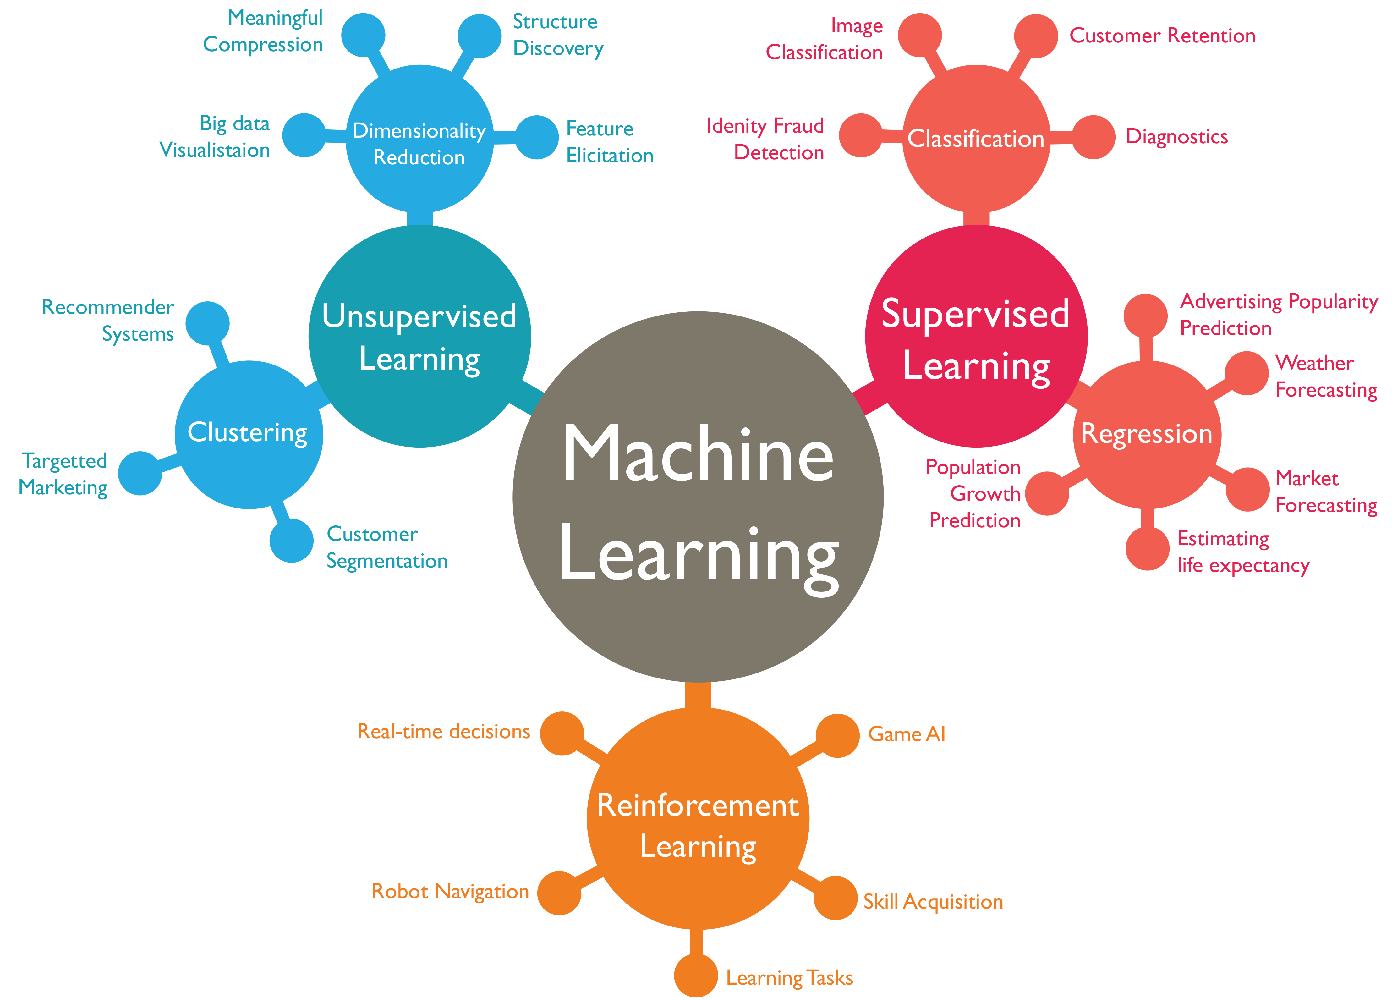
\includegraphics[width=0.8\textwidth]{ml_tasks.png}
		\caption{Overview Machine Learning Tasks}
		\citep{Artisan2020}
		\label{fig:ml_tasks}
	\end{figure} 

	\noindent It is shown in figure \ref{fig:ml_tasks}, that the main tasks for
	machine learning involve classification, regression, reinforcement
	learning, clustering and dimensionality reduction. This thesis focuses on 
	classification tasks. This task is chosen given the available data and 
	because it allows for a nice comparison of different machine learning models. 
	Well known standard machine learning models used for classification tasks 
	include logistic regression \citep{cramer2002origins}, naive bayes 
	\citep{zhang2004bayes}, support vector machines 
	\citep{platt1999probabilistic}, random forest classifiers
	\citep{breiman2001random}, AdaBoost \citep{freund1997decision} and
	artificial neural networks \citep{mcculloch1943logical}. This is an
	incomplete list of popular machine learning models that can be used for
	classification tasks. Popular applications of classification tasks include 
	predicting whether a customer is satisfied, whether to grant a mortgage 
	to a client and many more. The aforementioned machine learning methods have 
	in common, that they all only consider feature data and cannot consider 
	network information. \\

	\noindent Graph machine learning methods are different in that they consider 
	both feature data as well as network information. If one wants to categorize 
	graph machine learning within the framework shown in figure 
	\ref{fig:ml_overview}, it is probably best categorized as a special form of 
	neural network. It is however not a deep neural network, as network depth 
	does not necessarily improve the model and can be even counter-productive. 
	Within graph machine learning, there are two main approaches. The first 
	approach focuses on learning vector representations of graphs which are 
	used for downstream machine learning. The downstream machine learning models 
	include the standard models presented previously. Graph representation 
	learning approaches include models such as DeepWalk 
	\citep{perozzi2014deepwalk} and Node2Vec \citep{grover2016node2vec} among 
	others. The second approach involves the application of graph neural 
	networks for which there exist many different models. These networks 
	include models such as Graph Convolutional Networks \citep{kipf2016semi}, 
	GraphSage \citep{hamilton2017inductive} and many more. \\

	\noindent The detailed theoretical background for the considered graph
	machine learning models is provided in chapter 2.

	\section{Research Topic}
	\label{section:research_topics}

	\noindent The difficult access to graphs which also contain features, 
	motivate the search for alternatives. A review of the literature revealed, 
	that a form of synthetic graph generation could provide a solution to the data 
	access problem. Classic graph generation procedures include the famous 
	Erdös-Rényi graphs \citeyearpar{erdos1959random}, the small-world model by 
	\cite{watts1998collective}, the well-known model by 
	\cite{barabasi1999emergence} and more recently Kronecker Graphs by
	\cite{leskovec2010kronecker}. These models are all very instructive
	regarding the graph generation process and for understanding graph
	properties. These networks however all have the short-coming, that they do 
	not allow for the assignment of feature data to the nodes/observations in the
	network. It became clear, that one has to find or develop a model which 
	makes use of existing feature data for the graph generation process. 
	\cite{kim2012multiplicative} developed the \ac{mag} model. This model makes 
	use of randomly generated feature data which is referred to as attribute data 
	by the authors. The model is shown to be capable of generating random graphs 
	which can adhere to observed real world network properties. An analysis of 
	the \ac{mag} model reveals, that it could also be a useful model for 
	creating semi-synthetic graphs using existing feature data. For that reason, 
	the \ac{mag} model is selected for generating semi-synthetic graphs. This 
	model is introduced in detail in section \ref{section:theory_graphgen}. \\

	\noindent More recently, researchers have focused their attention to
	generative graph models. These models create graphs with features using
	real graphs as a training input. Examples for such models are graph
	\ac{rnn} \citep{you2018graphrnn} and deep generative graph
	models \citep{li2018learning}. These are very fascinating models which can
	be used to recreate or scale graph data. For the purpose of this thesis,
	these models are not purposeful, as it requires an existing graph with
	features to be available. Such a graph is unfortunately not available for
	this thesis. Nevertheless, this is an interesting current topic for graph 
	generation which was considered. \\ 

	\noindent The access problem to graphs which include feature data might be 
	resolved using the \ac{mag} model as previously mentioned. This model is 
	interesting as most researchers and companies have access to large amounts 
	of feature data such as customer databases or survey data. It would be of
	great benefit, if the available feature data could be used for generating
	semi-synthetic graphs. The \acs{mag} model provides a solution for
	generating such graphs. Semi-synthetic graph refers to the fact, that the 
	graph is generated using real feature data. Fully synthetic graphs on the 
	other hand are generated exclusively using artificial data. The goal of the
	semi-synthetic graph is to generate connections between the observations in 
	a given dataset. These connections should enhance the information present
	in the dataset. Graph machine learning should then be capable of exploiting
	these additional connections and hopefully provide competitive if not
	superior results compared to standard machine learning models. This thesis 
	therefore investigates to what extent semi-synthetic graphs can be used for 
	graph machine learning. Of course, semi-synthetic graphs are unlikely to be
	capable of fully substituting the performance of real graphs for machine 
	learning. Nevertheless, semi-synthetic graphs provide additional and 
	hopefully useful network information. To assess these hypotheses, the 
	results using graph machine learning are compared to standard machine 
	learning models. To close this section, the research question as well as the 
	hypotheses of this thesis are presented formally as follows. 

	\paragraph{Research Question}\mbox{}

	\noindent To what extent are semi-synthetic graphs based on real 
				feature data useful for a classification task using machine
				learning?

	\paragraph{Hypotheses}\mbox{}

	\noindent\textbf{H1:} Graph machine learning using semi-synthetic graphs
	provide superior results compared to the results of standard machine
	learning for a given classification task.\\

	\noindent\textbf{H2:} Graph machine learning using semi-synthetic graphs is
	a competitive strategy compared to the results of standard machine
	learning for a given classification task.\\


	\noindent The required theoretical background for this thesis which
	includes graph machine learning, graph generation and graph theory in
	general is provided in chapter 2.


  % Theory
  \chapter{Theory}
  
	This chapter will cover the necessary theoretical background for this
	master thesis and consists of following parts:

	\begin{enumerate}
		\item Graph Theory
		\item Machine Learning on Graphs
		\item Graph Generation
    \end{enumerate}

	\section{Graph Theory}

	This section provides a brief introduction to graph theory, with a focus on
	the relevant aspects for this master thesis. The theory presented is
	primarily taken from the book "Networks: An Introduction by Mark Newman
	\citeyearpar{Newman2010}. \\ 

	\noindent Graphs are special data structures as shown in Figure \ref{fig:graph}. The 
	terms graph and network are used inerchangeably for the purpose of this 
	master thesis. Typically, the term graph is used more commonly when referring 
	to mathematical analysis and the term network is more commonly used for data
	science purposes.

	\begin{figure}[h]
		\centering
		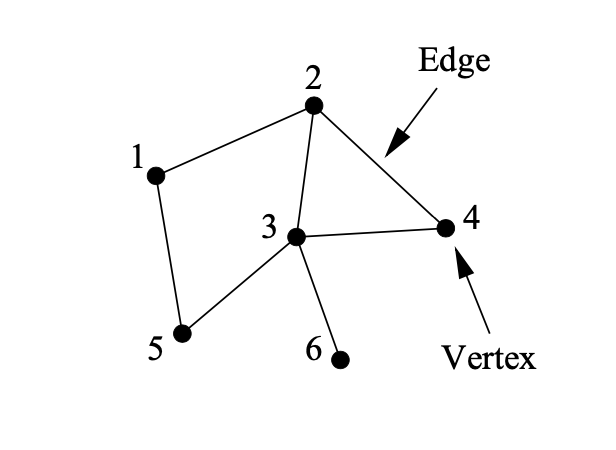
\includegraphics[width=0.5\textwidth]{graph.png}
		\caption{Example of a Graph}
		\cite[p. 111]{Newman2010}
		\label{fig:graph}
	\end{figure}
	
	\noindent The graph shown in Figure \ref{fig:graph} corresponds to an undirected graphs
	in which the connections between the vertexes are mutual. In a directed
	graph for instance, vertex A could be connected to vertex B, however vertex
	B need not be connected to vertex A. For the purpose of this thesis, only
	undirected graphs are considered. Vertexes are commonly reffered to as
	nodes and the terms will be used interchangeably. Edges refer to the
	connections between the vertices. Edges are often also referred to as links
	and the terms will be used interchangeably as well. Graphs may have
	additional elements such as multi-edges or self-edges. These are however
	not relevant for the purpose of this master thesis. \\

	\noindent In terms of mathematical notation, graphs are typically defined
	as follows:

	\begin{equation}
		G(V,E)
	\end{equation}

	\noindent $G$ refers to the graph as an output. $V$ refers to the set of 
	vertices present in the graph and $E$ refers to edges present between the 
	vertices. \\

	\subsection{Adjacency Matrix}

	The adjacency matrix $A$ is defined as a $n \times n$ matrix, where $n$ refers
	to the number of vertices present in the graph. Each vertex is therefore
	recorded by a column and a row in the adjacency matrix. The elements in the
	adjacency matrix are further typically defined as follows:

	\begin{equation}
		A_{ij} = 
			\begin{cases}
				1, & \text{if vertex $i$ and $j$ are connected by an edge} \\
				0, & \text{otherwise}
			\end{cases}
	\end{equation}
	
	\noindent For illustration, the adjacency matrix of the graph shown in Figure
	\ref{fig:graph} is shown as follows:

	\[ A = 
	\begin{pmatrix}
		0 & 1 & 0 & 0 & 1 & 0 \\
		1 & 0 & 1 & 1 & 0 & 0 \\
		0 & 1 & 0 & 1 & 1 & 1 \\
		0 & 1 & 1 & 0 & 0 & 0 \\
		1 & 0 & 1 & 0 & 0 & 0 \\
		0 & 0 & 1 & 0 & 0 & 0  
	\end{pmatrix}
	\] \\
	
	\noindent As one can see, if vertex $i$ and $j$ are connected, this is recorded with
	1 and 0 otherwise. Note, that all the elements on the $diag(A)$ are equal
	to 0. This is because self-edges are excluded. As this is an undirected
	network, the adjacency matrix is symmetric. There are many additonal
	aspects one could mention with regard to the adjacency matrix, they are
	however not relevant for this thesis.

	\subsection{Degree Measures}

	An important measure for graphs are the degrees $k$ of the vertices, the 
	number of edges connected to a vertex. The degrees of vertex $i$ can be 
	formulated as \citep[p.133]{Newman2010}:

	\begin{equation}
		k_i = \sum_{j=1}^{n} A_{ij}
	\end{equation}

	\noindent For an undirected graph, edges have two ends. This is due to the 
	fact that vertices connected by an edge are mutually connected. In terms of 
	the sum of the degrees of all vertices, we can therefore write for a graph 
	with $m$ edges \citep[p.133]{Newman2010}:

	\begin{equation}
		2m = \sum_{i=1}^{n} k_i	
	\end{equation}

	\noindent The sum of all degrees is therefore just the number of edges $m$ 
	multiplied by 2. In terms of statistical measures, the mean degree $c$ of a 
	vertex is defined as follows \citep[p.134]{Newman2010}:

	\begin{equation}
		c = \frac{1}{n}\sum_{i=1}^{n}k_i = \frac{2m}{n}
	\end{equation}

	\noindent In order to define the connectance or density of a graph, we must
	first observe, that the maximum number of edges is given by \citep[p.134]{Newman2010}:

	\begin{equation}
		{n \choose 2} = \frac{1}{2}n(n-1)
	\end{equation}

	\noindent The density $\rho$ can therefore be written as \citep[p.134]{Newman2010}:

	\begin{equation}
		\rho = \frac{m}{{n \choose 2}} = \frac{2m}{n(n-1)} = \frac{c}{n-1}
	\end{equation}

	\noindent Note, that the density $\rho$ lies strictly between 
	$0 \leqslant \rho \leqslant 1$. In addition, for sufficently large graphs,
	one can approximate $\rho = \frac{c}{n}$. 

	\subsection{Centrality Measures}

	The degrees of a vertex shown in the previous section already correspond to
	the simplest form of centrality measures. The issue with this measure
	however is, that the every neighbor of vertex $i$ are valued the same. This
	is a problem, as not all neigbors are of equalt importance due to:

	\begin{enumerate}
		\item Number of neighbors
		\item Importance of neighbor
		\item both
	\end{enumerate}

	\noindent There are many different alternative centrality measures which
	can consider the factors listed above such as eigenvector ecntrality, Katz
	centrality or PageRank
	\citep{katz1953new,page1999pagerank,landau1895relativen,Newman2010}. As we 
	are only dealing with simple undirected graphs, eigenvector centrality will 
	suffice, where the other mentioned methods are adaptations to the 
	eigenvector centrality. \\

	\noindent Eigenvector centrality gives all vertices a score proportional to
	the sum of the scores of its neighbors. This is a procedure in which
	typically the initial centrality $x_i$ of vertex $i$ is guessed to be 1
	$\forall \; i$. This can be used to calculate the centralities of the
	neighbors of $i$ which is denoted as $x_{i}'$. We can thus write
	\citep[p. 169]{Newman2010}:

	\begin{equation}
		x_i' = \sum_{j}A_{ij}x_j
	\end{equation}

	\noindent In matrix form:

	\begin{equation}
		x' = Ax
	\end{equation}

	\noindent This process is repeated $t$ times to provide better estimates
	\citep[p. 170]{Newman2010}:

	\begin{equation}
		x(t) =  A^tx(0)
	\end{equation}

	\noindent Where $x(0)$ is a linear combination of:

	\begin{equation}
		x(0) =  \sum_{i}c_{i}v_{i}
	\end{equation}

	\noindent $v_i$ correspond to the eigenvectors of the adjacency matrix $A$
	and $c_i$ corresponds to an appropriately chosen constant. 



	

	\section{Graph Generation}

	It is very difficult to collect graph data, as one cannot capture links
	between observations by traditional data collection means such as surveys. 
	In this regard, banks have a unique advantage (similar to social networks)
	in that they can capture relationships by analyzing their clients cash
	flows. In today's world most people make most if not all of their payments
	electronically and usually pay by card. This provides banks with a large
	amount of information such as spending behavior. Payments are nothing other
	than links in a graph theoretical setting. Unfortunately, access to bank
	client data is rarely granted due to privacy or bank secrecy laws. \\

	\noindent This is a problem for which no perfect solution exists. The
	search for alternatives lead to graph generation methods. Among the many 
	graph generation algorithms researched, the Multiplicative Attribute Graph 
	(MAG) modelappears to provide a feasible solution \citep{kim2012multiplicative}. 
	This model creates probabilistic links between observations using link-affinity
	matrices. 


  %\chapter{Chapter Three Title}
  %\input{chapters/chapter03}

  %\chapter{Chapter Four Title}
  %\input{chapters/chapter04}

  %\chapter{Conclusion}
  %
  This chapter includes the conclusion and provides an outlook for future
  research.

  \section{Conclusion}
  \label{section:conclusion}

  The aim of this thesis is to assess to what extent semi-synthetic graphs based 
  on real feature data are useful for machine learning. This aim corresponds to
  the research question stated in section \ref{section:research_topics}. The
  results for answering this question are mixed and are based on the data
  presented in chapter \ref{section:data}, the results of chapter
  \ref{section:results} and the discussion in chapter \ref{section:discussion}.
  \\

  \noindent Graph machine learning on the graph created from the Bank 
  Telemarketing dataset fails to overcome the problem of unbalanced labels. It 
  however yields similar results in terms of accuracy as the standard machine 
  learning models. In addition it is shown, that if a network structure can be 
  created which corresponds to the label, that the problem of unbalanced label 
  data could be overcome. \\

  \noindent GraphSage performs well for the US Airline Passenger dataset and
  is second only to the random forest classifier in terms of accuracy. As
  discussed, following the principle of Occam's razor, the good results for the
  GraphSage model must be taken with a grain of salt. For the purpose of
  gaining customer insights, simpler models such as ANN, SVM or AdaBoost provide
  only marginally inferior results and are more practical and thus preferable
  for this setting. Given similar results for more sensitive applications such
  as medicine, the GraphSage model could be preferred as even marginal
  performance improvements can be of utmost importance. In short, the GraphSage
  yields competitive results in terms of accuracy, the results are however not
  superior enough to necessarily warrant the complex graph generation process
  and model complexity of GraphSage. Lastly, the graph convolutional network and
  Node2Vec are not successful for the given classification task. For that
  reason more recent graph machine learning models should be tested and/or new 
  models should be developed to expand the possibilities of graph machine 
  learning.\\

  \noindent The perhaps most interesting result is provided by the US Airline
  Passenger graph plots shown in figure \ref{fig:us_airline_nodes}. The MAG 
  model successfully generates neighborhoods within the graph, where the nodes 
  are grouped according to their similarity which respects the similarities 
  between all attributes. This observation is further confirmed by the scatter 
  plots shown in figure \ref{fig:node2vec}. The graphs and the scatter plots
  make it possible to visually interpret the relationships within the data. 
  Standard scatter plots using the feature data do not allow for the generation 
  of such insightful graphs/plots. \\

  \noindent To summarize and provide an answer to the research question, it is
  shown that yes, semi-synthetic graphs can be useful for machine learning in a
  classification setting. The graph machine learning models are shown to be 
  competitive and could potentially even provide a solution for overcoming the 
  difficulties associated with unbalanced label data. This however requires the 
  availability of a graph with a structure which corresponds to the label. The 
  usefulness of semi-synthetic graphs are limited by the complexity associated 
  with generating graphs and the general complexity of graph machine learning 
  models. The graph based models further fail to outperform the standard machine 
  learning methods and are ranked anywhere between the second to fifth best 
  method depending on how one weights the trade off between model complexity 
  and accuracy. Based on this, the hypotheses presented in section
  \ref{section:research_topics} can be answered as follows: \\

  \noindent\textbf{H1:} Graph machine learning using semi-synthetic graphs fail
  to outperform standard machine learning methods. This hypothesis is thus
  rejected. \\

  \noindent\textbf{H2:} Graph machine learning is shown to be a competitive
  strategy with competitive results in line with the results shown for the
  standard machine learning methods. This hypothesis is not rejected.

  \section{Outlook}

  The discussion in chapter \ref{section:discussion} and the conclusion in section
  \ref{section:conclusion} provides interesting topics for future research.
  These topics include graph generation, cluster analysis on graphs and graph 
  machine learning models. 

  \paragraph{Graph Generation} \mbox{}
  
  \noindent Creating semi-synthetic graphs using the MAG method is shown to be a 
  viable method. The graph is however sensitive to attribute selection and 
  setting appropriate link-affinity probabilities. A fist step for resolving
  this issue was introduced by \cite{kim2011modeling} as a follow-up to their
  MAG model. In this paper they propose a reverse model, in which given a real
  graph, the attributes and the link-affinity probabilities are estimated such 
  that the attributes and link-affinity probabilities generate the observed real
  graph. This is however only a partial solution to the task given for this
  master's thesis. The estimated attributes do not correspond to real 
  attributes/features. In this model, the attributes are estimated to fit the 
  graph. An interesting topic for future research would be to develop a model 
  that generates a semi-synthetic graph based on attributes which at the same
  time optimizes link-affinity probabilities such that the resulting graph
  adheres to network properties observed in real graphs. Perhaps these more
  realistic graph properties can improve the performance for graph machine
  learning. This is an area worth consideration as especially the degree
  distribution and centrality measures shown in figure 
  \ref{fig:centrality_measures} force graph machine learning models to consider
  a large number of neighbors. In addition, even when sampling, the
  neighborhood is bound to always have the same size, given the range of the
  degree distribution shown in figure \ref{fig:centrality_measures}. This is a
  potential limiting factor for graph machine learning, as it potentially makes
  it more difficult to distinguish- and make use of different structures
  withing the graph.

  \paragraph{Cluster Analysis on Graphs} \mbox{}

  \noindent The graph plots shown in figure \ref{fig:us_airline_nodes} reveal,
  that semi-synthetic graphs can be excellent tools for visualizing data. The
  amount of useful information provided for interpreting the data is a welcome
  and unexpected result. For understanding the relationships between the
  attribute data and the label, the graph plots yielded the most useful
  information for identifying relationships within the data. An interesting
  topic for future research could be to assess how common clustering methods
  such as k-means, fuzzy clustering or CLIQUE could be used for analyzing
  graphs. Perhaps better and more graph centric methods could be developed. An
  excellent overview of existing graph clustering methods is provided by
  \cite{zhou2020graph}. Their article can be used as an initial reference point
  for identifying new applications of existing graph clustering methods or for 
  developing new models.

  \paragraph{Graph Machine Learning Models}\mbox{}

  \noindent Graph convolutional networks and GraphSage are selected for this
  thesis as they are probably the two most well-known GNNs. There are however 
  newer and more sophisticated models such as \ac{gat} \citep{velivckovic2018graph} 
  or \ac{gin} \citep{xu2019powerful}. \\

  \noindent GAT models have the ability of identifying more- or 
  less important neighbors in the graph. This is a useful ability and has been 
  shown to improve performance in some cases. This ability is unfortunately 
  most likely limited by the very large number of neighbors present in the US Airline 
  Passenger graph as shown in figure \ref{fig:centrality_measures}. For that
  reason, more realistic graphs with smaller number of degrees should be
  generated as suggested in the previous graph generation paragraph. \\

  \noindent GIN models are very well suited for distinguishing structures 
  within the graph. The authors \cite{xu2019powerful} present the general GIN
  framework which can accept any type of features as inputs whilst ensuring
  that the aggregation function is injective. Given the injective aggregation
  strategy, it is shown that the GIN can be as expressive at distinguishing
  graph structures as the Weisfeiler-Lehman graph isomorphism test 
  \citep{weisfeiler1968}. Again, for such a model to work best, the number of
  degrees would most likely need to be smaller than currently present in the
  graph of the US Airline Passenger dataset. Given the large number of degrees,
  the neighborhoods of every node are currently of the same size when using the
  sampling strategy outlined for the GraphSage model. \\

  \noindent Given a more realistic graph with a smaller number of degrees, it
  would be interesting to develop and assess, whether a new method which
  includes the attention mechanism of the GAT network with the isomorphic 
  capabilities of the GIN method could be of use. This new model could for
  instance be tested on well understood benchmark graphs such as Cora
  \citep{mccallum2000automating} or Citeseer \citep{giles1998citeseer}. 




  %%% endmatter
  \bibliography{bibliography.bib} 

  \appendix
  
  %\chapter{Appendix Title}
  %
  \section{Pairplot Feature Data}
  \label{App:pairplot}
  
  The pairplot of the feature data of the US Airline Passenger Data is shown in
  figure \ref{fig:pairplot_feature}.

  \begin{figure}[h]
		\centering
		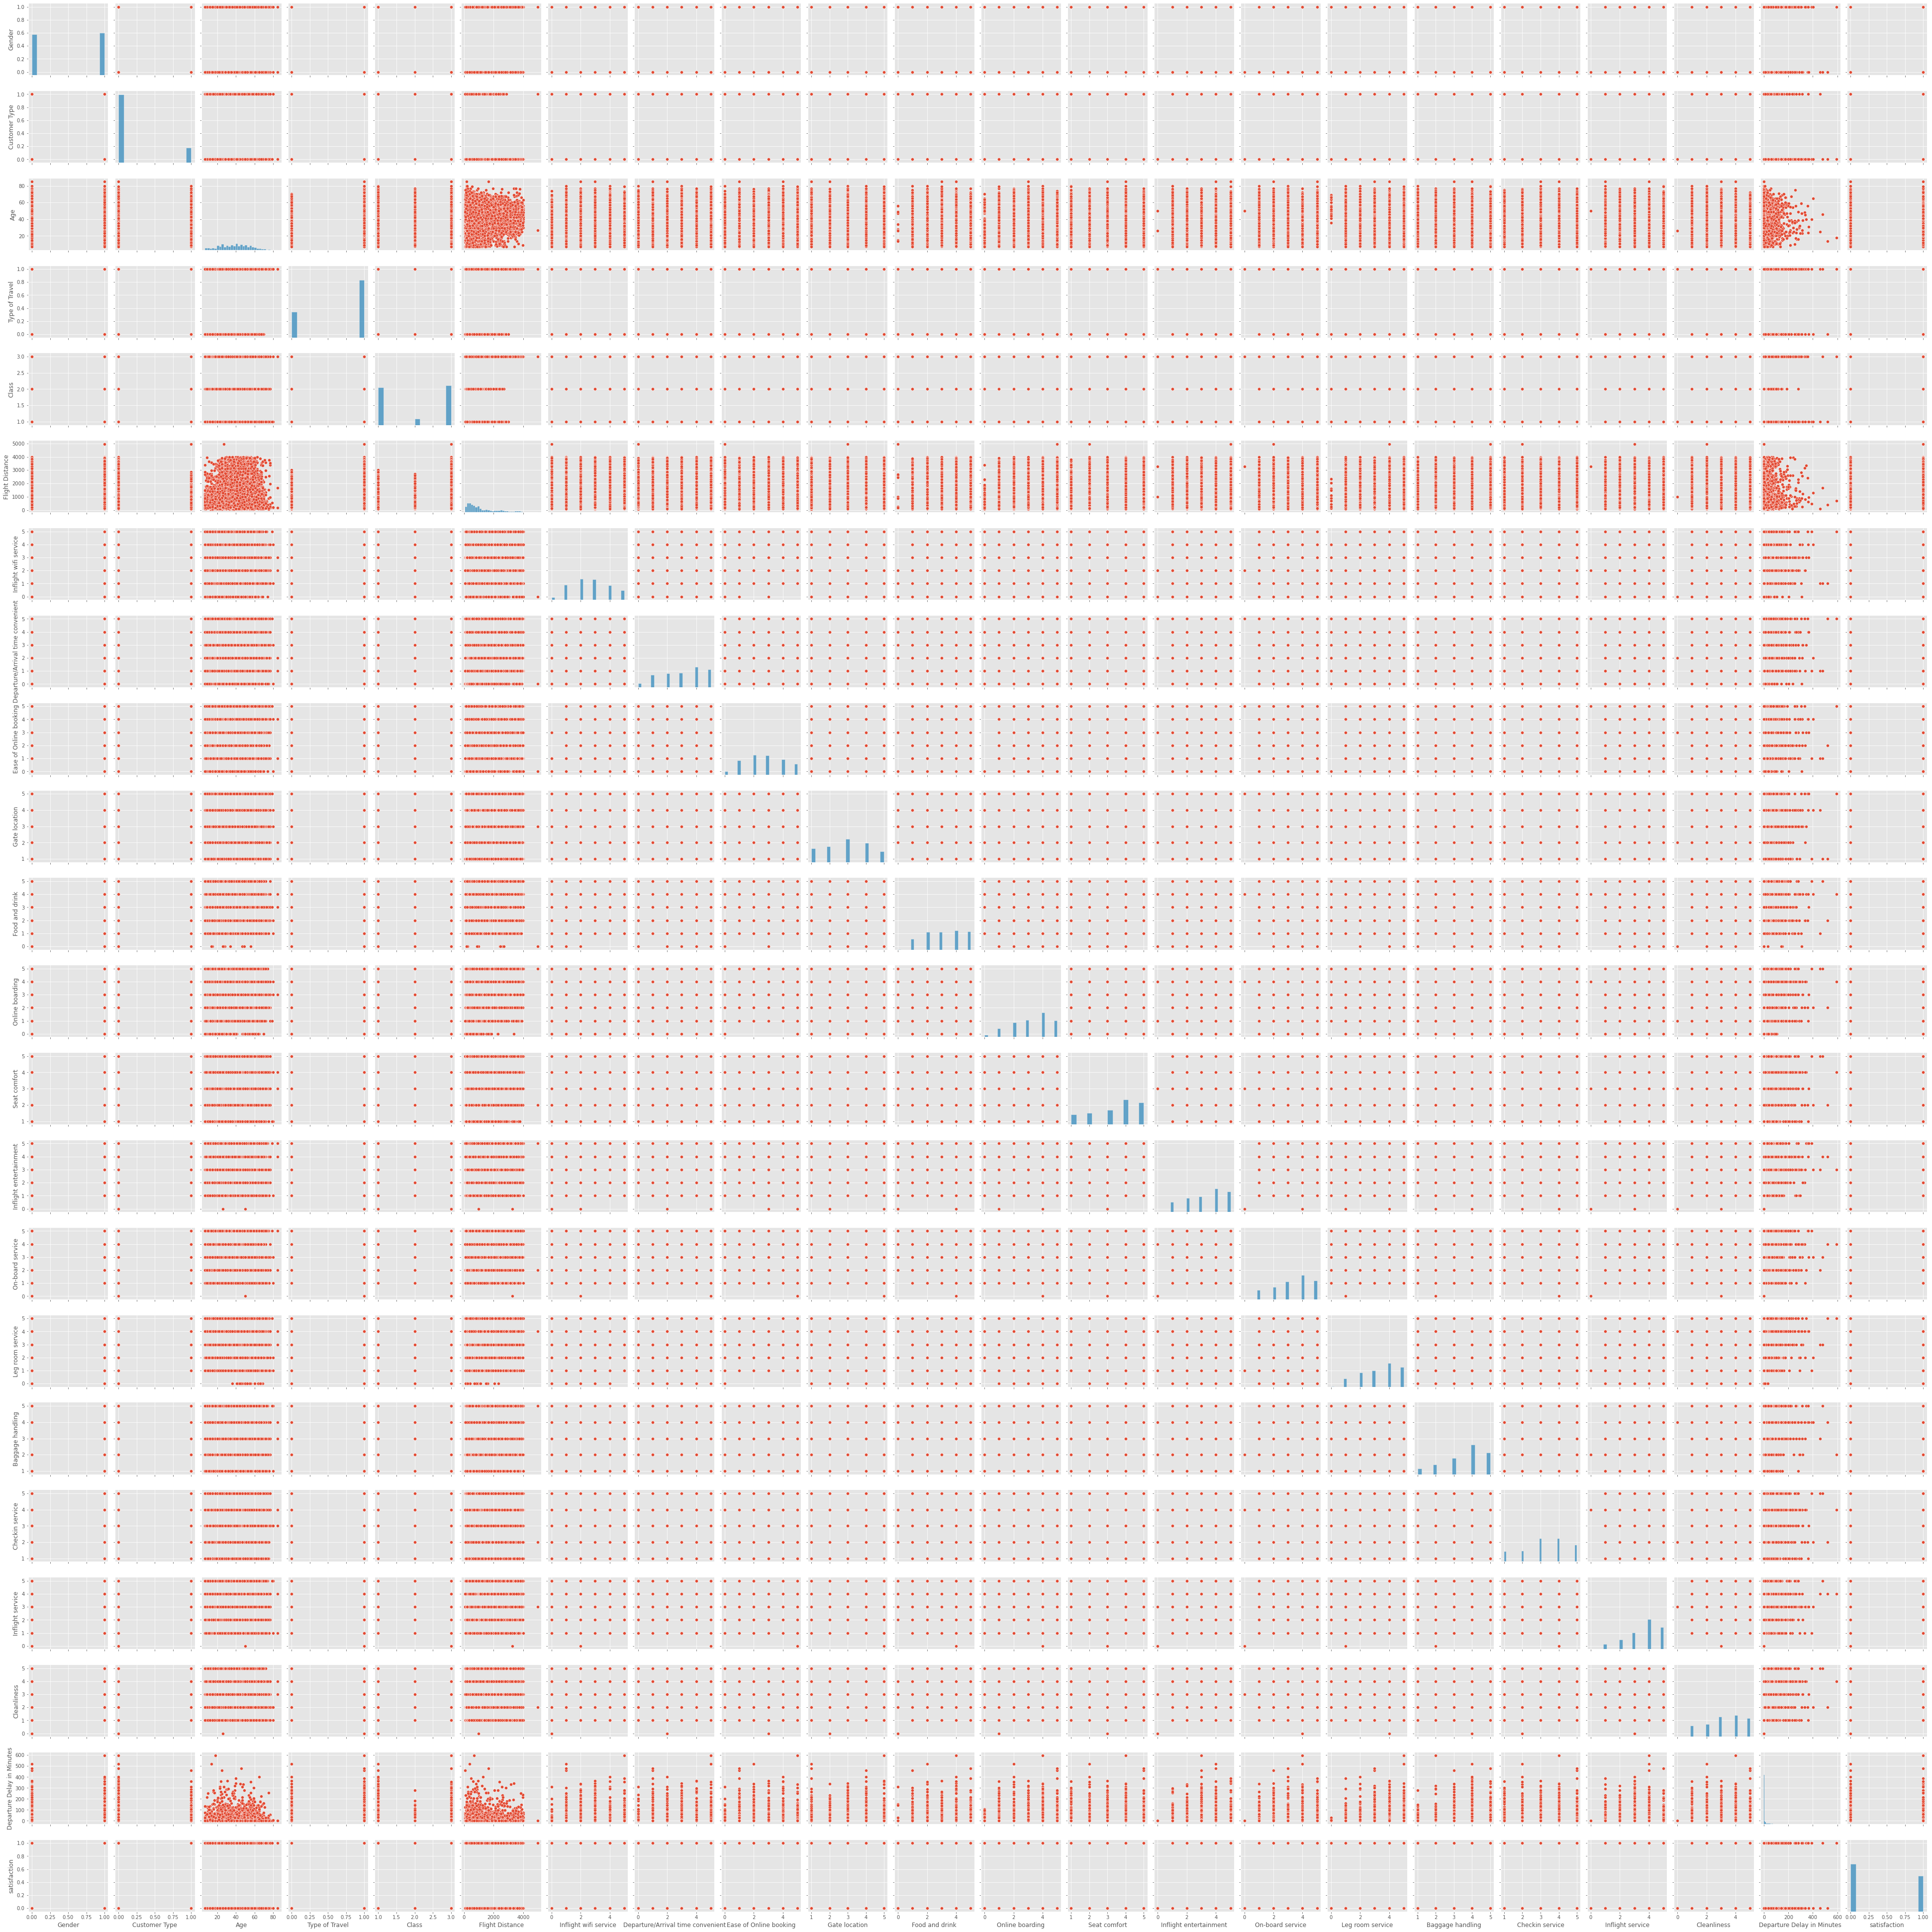
\includegraphics[width=0.9\textwidth]{pariplot_feature_data.png}
		\caption{Pairplot Feature Data US Airline Passenger Data Set}
        \label{fig:pairplot_feature}
  \end{figure}


\end{document}

